
%%%%%%%%%%%%%%%%
%%%%%%%%%%%%%%%%

\section{Biogeographic dating using DEC} \label{sec:bg_phylo}

This analysis will jointly estimate phylogeny and biogeography.
One benefit is that the biogeographic analysis will intrinsically accommodate phylogenetic uncertainty, both in terms of topology and branch lengths.
Another is that paleogeographic evidence has the potential provide information about the geological timing of speciation events in the phylogeny \citep{Ho2015}.
Finally, biogeographic data may lend support to certain phylogenetic relationships that have poor resolution otherwise.

As mentioned in Section \ref{sec:bg_simple}, Hawaiian silverswords are nested within the subtribe {\it Madiinae}, alongside the tarweeds, a clade of plants inhabiting in western North America.
Fossil pollen evidence indicates that {\it Madiinae} diversified during a period of aridification from 15--5 Ma in the western regions of North America \citep{Baldwin1991}.
It's clear that silverswords colonized Hawaii from western North America, but the timing of the event is difficult to estimate.
Even though the oldest Hawaiian island they inhabit is Kauai, it is possible that silverswords first colonized older islands in the Emperor Island chain that predate the formation of Kauai (ca 5.1 Ma).

This makes the application of standard node-based biogeographic calibrations challenging, because it would require a strong assumption about when and how many times the oldest silversword lineages colonized Kauai.
Did silverswords colonize Kauai once directly from the California coast? Or did the colonize the younger islands multiple times from older islands in the chain? And did the event occur immediately after Kauai surfaced or much later? Because we cannot observe the timing and nature of this event directly, we will integrate over all possible evolutionary histories using process-based biogeographic dating method described in \citet{Landis2016}.

\begin{figure}[!h]
\centering
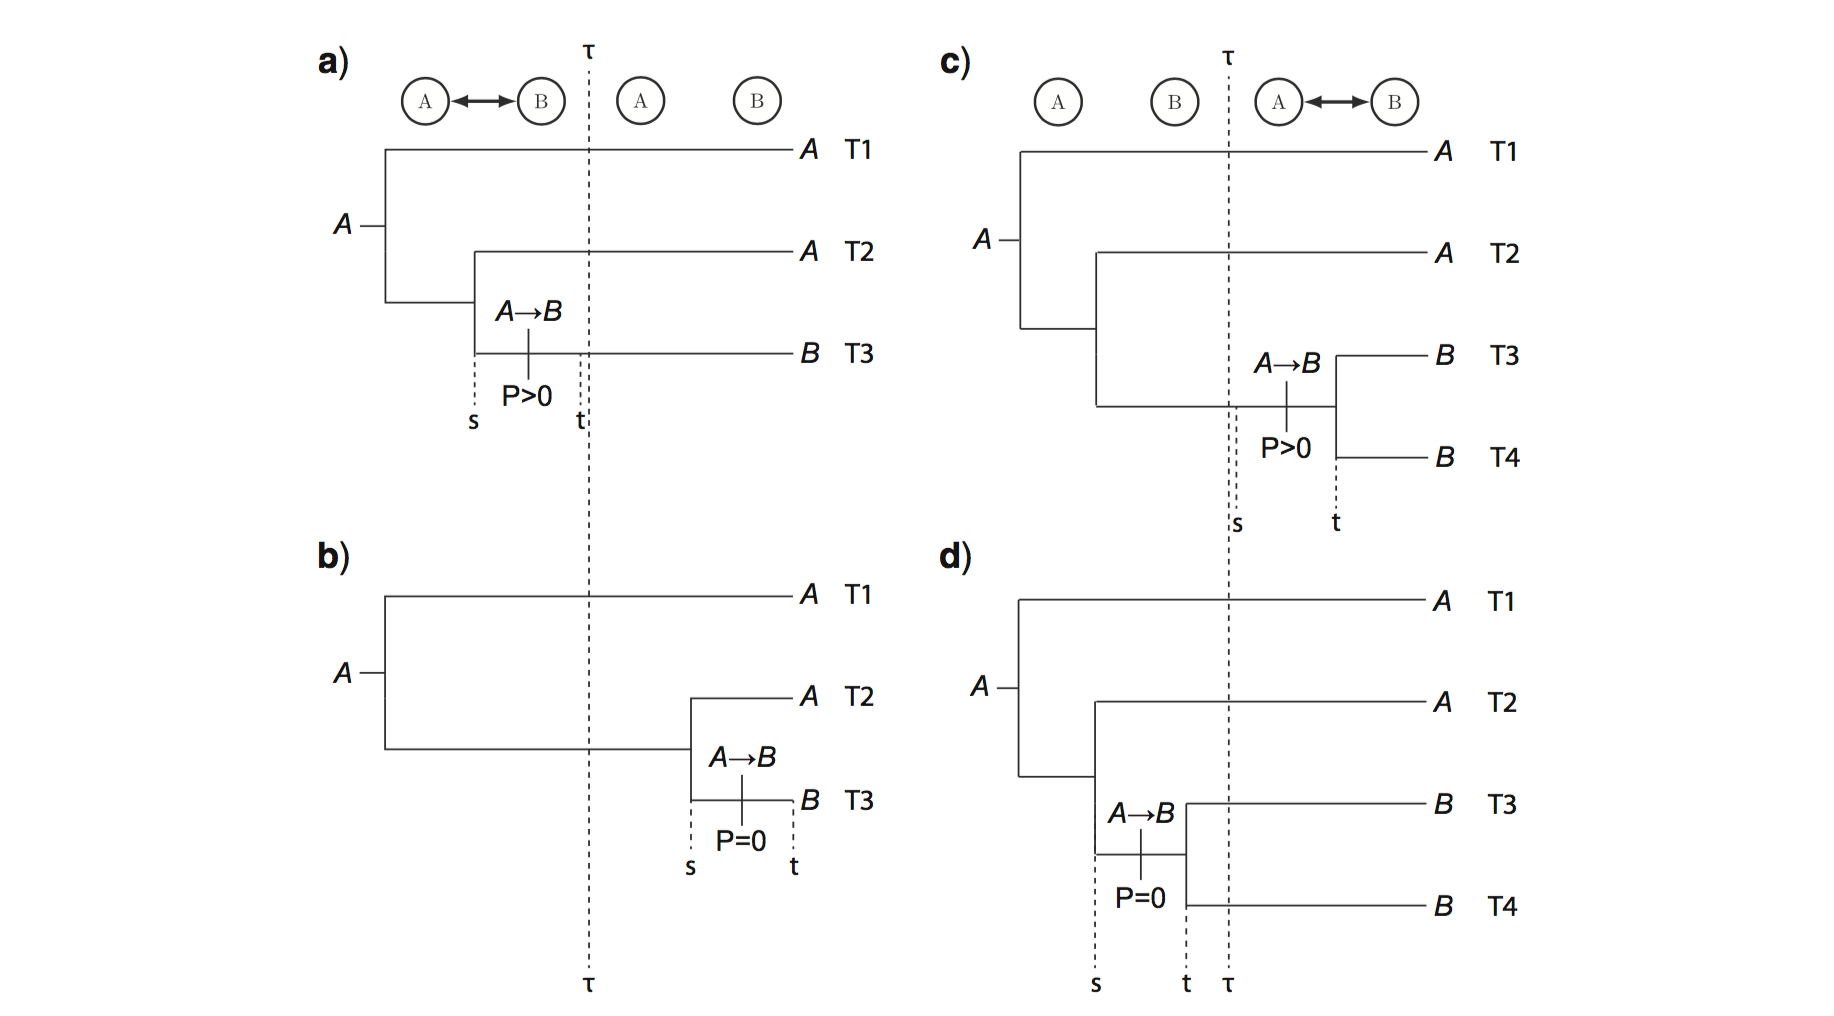
\includegraphics[width=0.8\textwidth]{figures/fig_biogeo_dating.png}
\caption{Cartoon of biogeographic transition probabilities as functions of geological time, and how that relates to speciation times. (a) Areas split, dispersal before split, positive probability; (b) Areas split, dispersal after split, zero probability; (c) Areas merge, dispersal after merge, positive probability; (d) Areas merge, dispersal before merge, zero probabilty. Original figure and details regarding cartoon assumptions are found in \citet{Landis2016}.}
\label{fig:biogeo_dating_cartoon}
\end{figure}

The basic idea is that an empirically informed epoch model is capable of creating conditions that favor key evolutionary transitions to occur during one time interval over another.
Unlike the time-homogeneous probabilities that arise from, say, a molecular substitution process, these age-dependent transition probabilities may identify rate from time, and thus generate information about branch lengths in units of absolute time (Figure \ref{fig:biogeo_dating_cartoon}).
A biogeographic process that is constrained by paleogeographic connectivity is well-suited to this purpose.

Note: like all dating methods, including node calibration methods, tip dating methods, and fossilized birth death dating methods, process-based biogeographic dating estimates are prior sensitive and dataset dependent.
Applying this model to alternative data sets should be done with care!

Much of this tutorial will be similar to the previous sections, except we are adding a birth-death process and a molecular substitution process to the model graph.

\subsection{Analysis}

To use date the silversword radiation using biogeography, it is necessary that we transition from our simpler 4-area model to a richer 6-area model (see Figure \ref{fig:hawaii_areas}).
The mainland area (Z) is necessary to force the silversword and tarweed clade to originate apart from the islands.
The area corresponding to the older island chain (R) is necessary because we do not know {\it a priori} whether silverswords colonized the modern islands directly from the mainland (Z $\rightarrow$ K), or first colonized R and only later dispersed into the younger islands any number of times (Z $\rightarrow$ R $\rightarrow$ K).
Thus, adding these two areas allows the silversword origin time to precede the formation of Kauai when the dispersal rate is large.

Additionally, we will add three tarweed taxa to our dataset, increasing the total number of taxa to 38.
We'll use a molecular alignment for the internal transcribed spacer (ITS) to estimate the phylogeny, which is a 657bp non-coding locus that is historically important for plant systematics.
Because the locus is relatively short, it will also leave us with a fair amount of phylogenetic uncertainty in branch length and topology estimates.
However, because we're estimating phylogeny and biogeography, it will be correctly incorporated into our ancestral range estimates.

As usual, we'll begin by creating variables to manage our input and output files

\begin{snugshade}
\begin{lstlisting}
range_fn = "data/n6/silversword.n6.range.nex"
mol_fn = "data/n6/silversword.mol.nex"
tree_fn = "data/n6/silversword.tre"
out_fn = "output/test_epoch_phy"
geo_fn = "data/n6/hawaii.n6"
times_fn = geo_fn + ".times.txt"
dist_fn = geo_fn + ".distances.txt"
\end{lstlisting}
\end{snugshade}

Add the analysis helper variables

\begin{snugshade}
\begin{lstlisting}
mvi = 1
mni = 1
n_gen = 1e5    # more parameters, longer run!
\end{lstlisting}
\end{snugshade}


Read in the molecular alignment

\begin{snugshade}
\begin{lstlisting}
dat_mol = readDiscreteCharacterData(mol_fn)
\end{lstlisting}
\end{snugshade}


Read in the species ranges for six areas

\begin{snugshade}
\begin{lstlisting}
dat_range_01 = readDiscreteCharacterData(range_fn)
\end{lstlisting}
\end{snugshade}

Compute the number of ranges when ranges may only be one or two areas in size

\begin{snugshade}
\begin{lstlisting}
n_areas <- dat_range_01.nchar()
max_areas <- 2
n_states <- 0
for (k in 0:max_areas) n_states += choose(n_areas, k)
\end{lstlisting}
\end{snugshade}

Then format the dataset for the reduced state space

\begin{snugshade}
\begin{lstlisting}
dat_range_n = formatDiscreteCharacterData(dat_range_01, "DEC", n_states)
\end{lstlisting}
\end{snugshade}

Record the complete list of range descriptions to file

\begin{snugshade}
\begin{lstlisting}
state_desc = dat_range_n.getStateDescriptions()
state_desc_str = "state,range\n"
for (i in 1:state_desc.size())
{
    state_desc_str += (i-1) + "," + state_desc[i] + "\n"
}
write(state_desc_str, file=out_fn+".state_labels.txt")
\end{lstlisting}
\end{snugshade}

Read the minimum and maximum ages of the island complexes

\begin{snugshade}
\begin{lstlisting}
time_bounds <- readDataDelimitedFile(file=times_fn, delimiter=" ")
n_epochs <- time_bounds.size()
\end{lstlisting}
\end{snugshade}

Read in the connectivity matrices between the six areas

\begin{snugshade}
\begin{lstlisting}
for (i in 1:n_epochs) {
  epoch_fn[i] = geo_fn + ".connectivity." + i + ".txt"
  connectivity[i] <- readDataDelimitedFile(file=epoch_fn[i], delimiter=" ")
}
\end{lstlisting}
\end{snugshade}

Read the geographical distances between areas

\begin{snugshade}
\begin{lstlisting}
distances <- readDataDelimitedFile(file=dist_fn, delimiter=" ")
\end{lstlisting}
\end{snugshade}

Remember that we are estimating the phylogeny as part of this analysis.
In general, it is possible that certain combinations of phylogeny, biogeography, and paleogeography have zero-valued likelihoods should the epoch model introduce reducible rate matrix structures \citep[see the supplemental of][]{Buerki2011}.
The initial MCMC state, however, must have a non-zero probability for it to work properly.
Although it may not be needed, we will provide {\tt tree\_init} as a starting tree for the {\tt tree} variable that we will create to be safe.

\begin{snugshade}
\begin{lstlisting}
tree_init = readTrees(tree_fn)[1]
\end{lstlisting}
\end{snugshade}

We will record some basic information about the taxon set, the number of taxa, and the number of branches in the tree

\begin{snugshade}
\begin{lstlisting}
taxa = tree_init.taxa()
n_taxa = taxa.size()
n_branches = 2 * n_taxa - 2
\end{lstlisting}
\end{snugshade}

\subsubsection{The tree model}

Because we will estimate the topology and branch lengths parameters, the {\tt tree} variable must be declared as a stochastic node with a prior distribution.
For this, we'll use a constant rate birth-death process.

Assign root age with a maximum age of 15Ma to reflect the fossil pollen record for Californian tarweeds \citep{Baldwin1998}. No assumption is made about the minimum root age.

\begin{snugshade}
\begin{lstlisting}
root_age ~ dnUniform(0, 15)
moves[mvi++] = mvScale(root_age, weight=2)
\end{lstlisting}
\end{snugshade}

Assign the proportion of sampled taxa (we have a non-uniform sampling scheme, but this should suffice).

\begin{snugshade}
\begin{lstlisting}
rho <- 35/50
\end{lstlisting}
\end{snugshade}

Assign the birth and death priors.
It is important to note that the birth and death priors induce a root age distribution through the birth-death process.
These priors generate a relatively uniform root age distribution between 2.5--15 Ma in the absence of data (i.e. running MCMC with the {\tt underPrior=true} option).
\begin{snugshade}
\begin{lstlisting}
birth ~ dnExp(1)
moves[mvi++] = mvScale(birth)
death ~ dnExp(1)
moves[mvi++] = mvScale(death)
\end{lstlisting}
\end{snugshade}

Instantiate a tree variable generated by a birth-death process
\begin{snugshade}
\begin{lstlisting}
tree ~ dnBDP(lambda=birth, mu=death, rho=rho, rootAge=root_age, taxa=taxa)
\end{lstlisting}
\end{snugshade}


Add topology and branch length moves
\begin{snugshade}
\begin{lstlisting}
moves[mvi++] = mvNNI(tree, weight=n_branches/2)
moves[mvi++] = mvFNPR(tree, weight=n_branches/8)
moves[mvi++] = mvNodeTimeSlideUniform(tree, weight=n_branches/2)
\end{lstlisting}
\end{snugshade}

Provide a starting tree to ensure the biogeographic model has non-zero likelihood

\begin{snugshade}
\begin{lstlisting}
tree.setValue(tree_init)
root_age.setValue(tree_init.rootAge())
\end{lstlisting}
\end{snugshade}


\subsubsection{The molecular model}

To inform our branch lengths (in relative time units) and our topology, we will specify a simple HKY+$\Gamma4$+UCLN model of molecular substitution \citep{Hasegawa1985,Yang1998,Drummond2006}.

First specify a base rate for the molecular clock.
This prior is uniform over orders of magnitude, between $10^{-6}$ and $10^3$, and was chosen to minimize its influence on the tree height.

\begin{snugshade}
\begin{lstlisting}
log10_rate_mol ~ dnUniform(-6, 3)
log10_rate_mol.setValue(-1)
moves[mvi++] = mvSlide(log10_rate_mol, weight=5, delta=0.2)
rate_mol := 10^log10_rate_mol
\end{lstlisting}
\end{snugshade}

Assign log-normal relaxed clock rate multipliers to each branch in the tree.
These priors have a mean of 1 so each branch prefers a strict clock model in the absence of data.
\begin{snugshade}
\begin{lstlisting}
branch_sd <- 1.0
branch_mean <- 0.0 - 0.5 * branch_sd^2
for (i in 1:n_branches) {
    branch_rate_multiplier[i] ~ dnLognormal(mean=branch_mean, sd=branch_sd)
    moves[mvi++] = mvScale(branch_rate_multiplier[i])
    branch_rates[i] := rate_mol * branch_rate_multiplier[i]
}
\end{lstlisting}
\end{snugshade}

Now we'll create an HKY rate matrix.
First, we create a Gamma-distributed transition-transversion (Ts/Tv) rate ratio with prior with mean equal to one

\begin{snugshade}
\begin{lstlisting}
kappa ~ dnGamma(2,2)
moves[mvi++] = mvScale(kappa)
\end{lstlisting}
\end{snugshade}

then create a flat Dirichlet prior on the base frequencies over A, C, G, and T

\begin{snugshade}
\begin{lstlisting}
bf ~ dnDirichlet([1,1,1,1])
moves[mvi++] = mvSimplexElementScale(bf, alpha=10, weight=2)
\end{lstlisting}
\end{snugshade}

and, finally, combine the base frequencies and Ts/Tv rate ratio to build the rate matrix

\begin{snugshade}
\begin{lstlisting}
Q_mol := fnHKY(kappa, bf)
\end{lstlisting}
\end{snugshade}

Next, we'll create a $+\Gamma4$ across-site rate variation model.
First, we need a parameter to control the amount of site rate variation

\begin{snugshade}
\begin{lstlisting}
alpha ~ dnUniform(0,50)
moves[mvi++] = mvScale(alpha)
\end{lstlisting}
\end{snugshade}

and a discretized Gamma distribution with four categories

\begin{snugshade}
\begin{lstlisting}
site_rates := fnDiscretizeGamma(alpha, alpha, 4)
\end{lstlisting}
\end{snugshade}

The distribution of site rates categories has mean equal to one and variance equal to $1/\alpha$.
When {\tt alpha} grows small, the amount of site rate heterogeneity increases.
When {\tt alpha} is large, the variance shrinks to zero, and the site rate multipliers of {\tt site\_rates} converge to the value 1.

Finally, we'll create our molecular model of substitution

\begin{snugshade}
\begin{lstlisting}
m_mol ~ dnPhyloCTMC(Q=Q_mol, tree=tree, branchRates=branch_rates, siteRates=site_rates, type="DNA", nSites=dat_mol.nchar())
\end{lstlisting}
\end{snugshade}

and attach the ITS alignment

\begin{snugshade}
\begin{lstlisting}
m_mol.clamp(dat_mol)
\end{lstlisting}
\end{snugshade}


\subsubsection{The biogeographic model}
% distances between areas

The biogeographic model is identical to that described in Section \ref{sec:bg_epoch}, so redundant details are omitted here.

First, create the biogeographic rate parameter.

\begin{snugshade}
\begin{lstlisting}
log10_rate_bg ~ dnUniform(-4,2)
log10_rate_bg.setValue(-2)
rate_bg := 10^log10_rate_bg
moves[mvi++] = mvSlide(log10_rate_bg, weight=4)
\end{lstlisting}
\end{snugshade}


The relative dispersal rate is fixed to 1
\begin{snugshade}
\begin{lstlisting}
dispersal_rate <- 1.0
\end{lstlisting}
\end{snugshade}


the distance scale parameter

\begin{snugshade}
\begin{lstlisting}
distance_scale ~ dnUnif(0,20)
distance_scale.setValue(0.001)
moves[mvi++] = mvScale(distance_scale, weight=3)
\end{lstlisting}
\end{snugshade}


Next, create dispersal rates that are functions of distance between all pairs of areas, but between areas that exist during epoch {\tt i}!

%dr[i][j][k] := (a * exp( -b * distances[j][k] ))
\begin{snugshade}
\begin{lstlisting}
for (i in 1:n_epochs) {
  for (j in 1:n_areas) {
    for (k in 1:n_areas) {
     dr[i][j][k] <- 0.0
     if (connectivity[i][j][k] > 0) {
       dr[i][j][k] := dispersal_rate * exp(-distance_scale * distances[j][k])
     }
    }
  }
}
\end{lstlisting}
\end{snugshade}


% extirpation penalized ranges
% ... they can exist, but not persist

Create the extirpation rates

\begin{snugshade}
\begin{lstlisting}
log_sd <- 0.5
log_mean <- ln(1) - 0.5*log_sd^2
extirpation_rate ~ dnLognormal(mean=log_mean, sd=log_sd)
moves[mvi++] = mvScale(extirpation_rate, weight=2)

for (i in 1:n_epochs) {
  for (j in 1:n_areas) {
    for (k in 1:n_areas) {
      er[i][j][k] <- 0.0
    }
    er[i][j][j] := extirpation_rate
  }
}

\end{lstlisting}
\end{snugshade}


Build a rate matrix for each time interval
\begin{snugshade}
\begin{lstlisting}
for (i in 1:n_epochs) {
  Q_DEC[i] := fnDECRateMatrix(dispersalRates=dr[i],
                          extirpationRates=er[i],
                          maxRangeSize=max_areas)
}
\end{lstlisting}
\end{snugshade}


Treat epoch times as random variables, except the present is always the present (or is it?).

\begin{snugshade}
\begin{lstlisting}
for (i in 1:n_epochs) {
  time_max[i] <- time_bounds[i][1]
  time_min[i] <- time_bounds[i][2]
  if (i != n_epochs) {
    epoch_times[i] ~ dnUniform(time_min[i], time_max[i])
    moves[mvi++] = mvSlide(epoch_times[i], delta=(time_bounds[i][1]-time_bounds[i][2])/2)
  } else {
    epoch_times[i] <- 0.0
  }
}
\end{lstlisting}
\end{snugshade}

Wrap the vector of rate matrices with the {\tt fnEpoch} rate generator function

\begin{snugshade}
\begin{lstlisting}
Q_DEC_epoch := fnEpoch(Q=Q_DEC, times=epoch_times, rates=rep(1, n_epochs))
\end{lstlisting}
\end{snugshade}

% clado event probs

Here, we treat the probability of different types of cladogenetic events as a random variable to be estimate.

\begin{snugshade}
\begin{lstlisting}
clado_event_types <- [ "s", "a" ]
p_sympatry ~ dnUniform(0,1)
p_allopatry := abs(1.0 - p_sympatry)
moves[mvi++] = mvSlide(p_sympatry, delta=0.1, weight=2)
clado_event_probs := simplex(p_sympatry, p_allopatry)
P_DEC := fnDECCladoProbs(eventProbs=clado_event_probs,
                         eventTypes=clado_event_types,
                         numCharacters=n_areas,
                         maxRangeSize=max_areas)
\end{lstlisting}
\end{snugshade}

Based on fossil pollen evidence, force range state and the root of the tree to be the mainland area (Z)

\begin{snugshade}
\begin{lstlisting}
rf_DEC <- rep(0, n_states)
rf_DEC[n_areas+1] <- 1  # Mainland (Z) is the only possible starting state
rf_DEC <- simplex(rf_DEC)
\end{lstlisting}
\end{snugshade}


Create the phylogenetic model of range evolution

\begin{snugshade}
\begin{lstlisting}
m_bg ~ dnPhyloCTMCClado(tree=tree,
                           Q=Q_DEC_epoch,
                           cladoProbs=P_DEC,
                           branchRates=rate_bg,
                           rootFrequencies=rf_DEC,
                           type="NaturalNumbers",
                           nSites=1)        
\end{lstlisting}
\end{snugshade}


Attach the species range dataset to the model

\begin{snugshade}
\begin{lstlisting}
m_bg.clamp(dat_range_n)
\end{lstlisting}
\end{snugshade}


To easily identify interactions between the posterior estimates of island ages and divergence times, we'll create a deterministic node to monitor the age of the silversword radiation.
First, create a deterministic node to monitor the crown age of the silversword radiation

\begin{snugshade}
\begin{lstlisting}
ingroup_clade <- clade("Wilkesia_hobdyi",
                       "Dubautia_reticulata",
                       "Dubautia_microcephala",
                       "Argyroxiphium_caliginis")

ingroup_age := tmrca(tree, ingroup_clade)
\end{lstlisting}
\end{snugshade}

Next, create a vector of variables to report the posterior probability that the clade originates {\it before} a given island.
When the first argument in of the {\tt ifelse} function returns {\tt true}, the node has value {\tt 1} and {\tt 0} otherwise.
Thus, the mean of this variable gives the posterior probability that the inequality is satisfied.

\begin{snugshade}
\begin{lstlisting}
for (i in 1:n_epochs) {
  ingroup_older_island[i] := ifelse(ingroup_age > epoch_times[i], 1, 0)
}
\end{lstlisting}
\end{snugshade}

Create the standard monitors.
One difference is that the {\tt mnFile} monitor will now record the posterior distribution for the {\tt tree} variable, whereas the previous two tutorials assumed {\tt tree} was fixed.

\begin{snugshade}
\begin{lstlisting}
monitors[mni++] = mnScreen(printgen=100, ingroup_age)
monitors[mni++] = mnModel(file=out_fn+".model.log", printgen=100)
monitors[mni++] = mnFile(tree, filename=out_fn+".tre", printgen=100)
monitors[mni++] = mnJointConditionalAncestralState(tree=tree,
                                                       ctmc=m_bg,
                                                       type="NaturalNumbers",
                                                       withTips=true,
                                                       withStartStates=true,
                                                       filename=out_fn+".states.log",
                                                       printgen=100)
\end{lstlisting}
\end{snugshade}


Because {\tt ingroup\_older\_island} does not contribute to the model likelihood, it must be manually introduced to the model object.
Compose the model object.

\begin{snugshade}
\begin{lstlisting}
mymodel = model(m_bg, ingroup_older_island)
\end{lstlisting}
\end{snugshade}

Create the MCMC object and run the analysis.

\begin{snugshade}
\begin{lstlisting}
mymcmc = mcmc(mymodel, moves, monitors)
mymcmc.run(n_gen)
\end{lstlisting}
\end{snugshade}

\begin{figure}[!h]
\centering
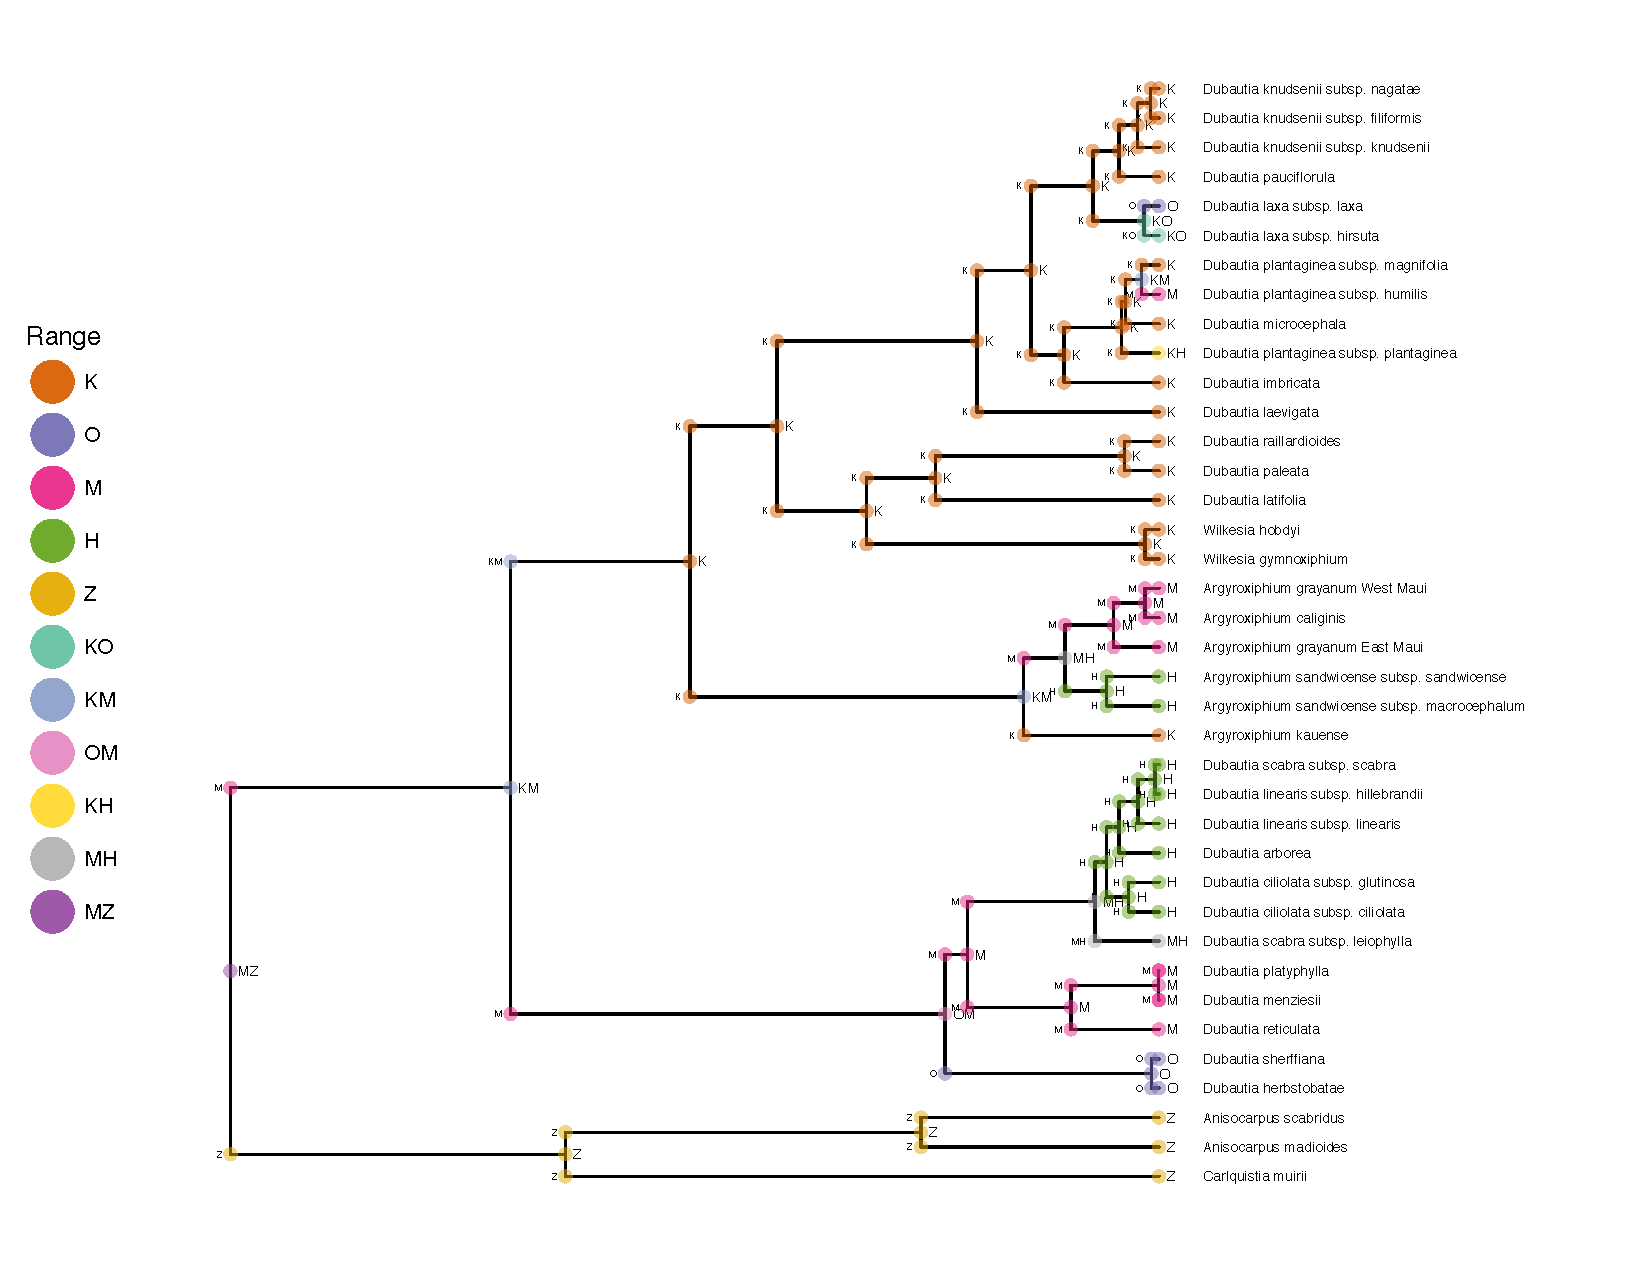
\includegraphics[width=0.8\textwidth]{figures/fig_simple_phy_RevGadgets_ase.pdf}
\caption{Joint estimate of phylogeny and biogeography, ignoring paleogeography.}
\label{fig:simple_phy}
\end{figure}

\subsection{Results}

\begin{center}
{\it Example results are located at \tt{output\_example/epoch\_phy.*} and \tt{output\_example/simple\_phy.*} }
\end{center}

To understand the influence of the epoch model on ancestral range and divergence time estimation, it is important to run addition analyses with alternative settings.
Scripts to jointly estimate molecular evolution, historical biogeographic, and phylogenetic parameters are available as {\tt scripts/run\_simple\_phy.Rev} and {\tt scripts/run\_epoch\_phy.Rev}.
The ``epoch'' analysis is identical to the analysis just described.
The ``simple'' analysis is similar to the ``epoch'' analysis, except it substitutes the paleogeography-aware model of range evolution (see Section \ref{sec:bg_epoch}) for a paleogeography-naive model (see Section \ref{sec:bg_simple}).

\begin{figure}[!h]
\centering
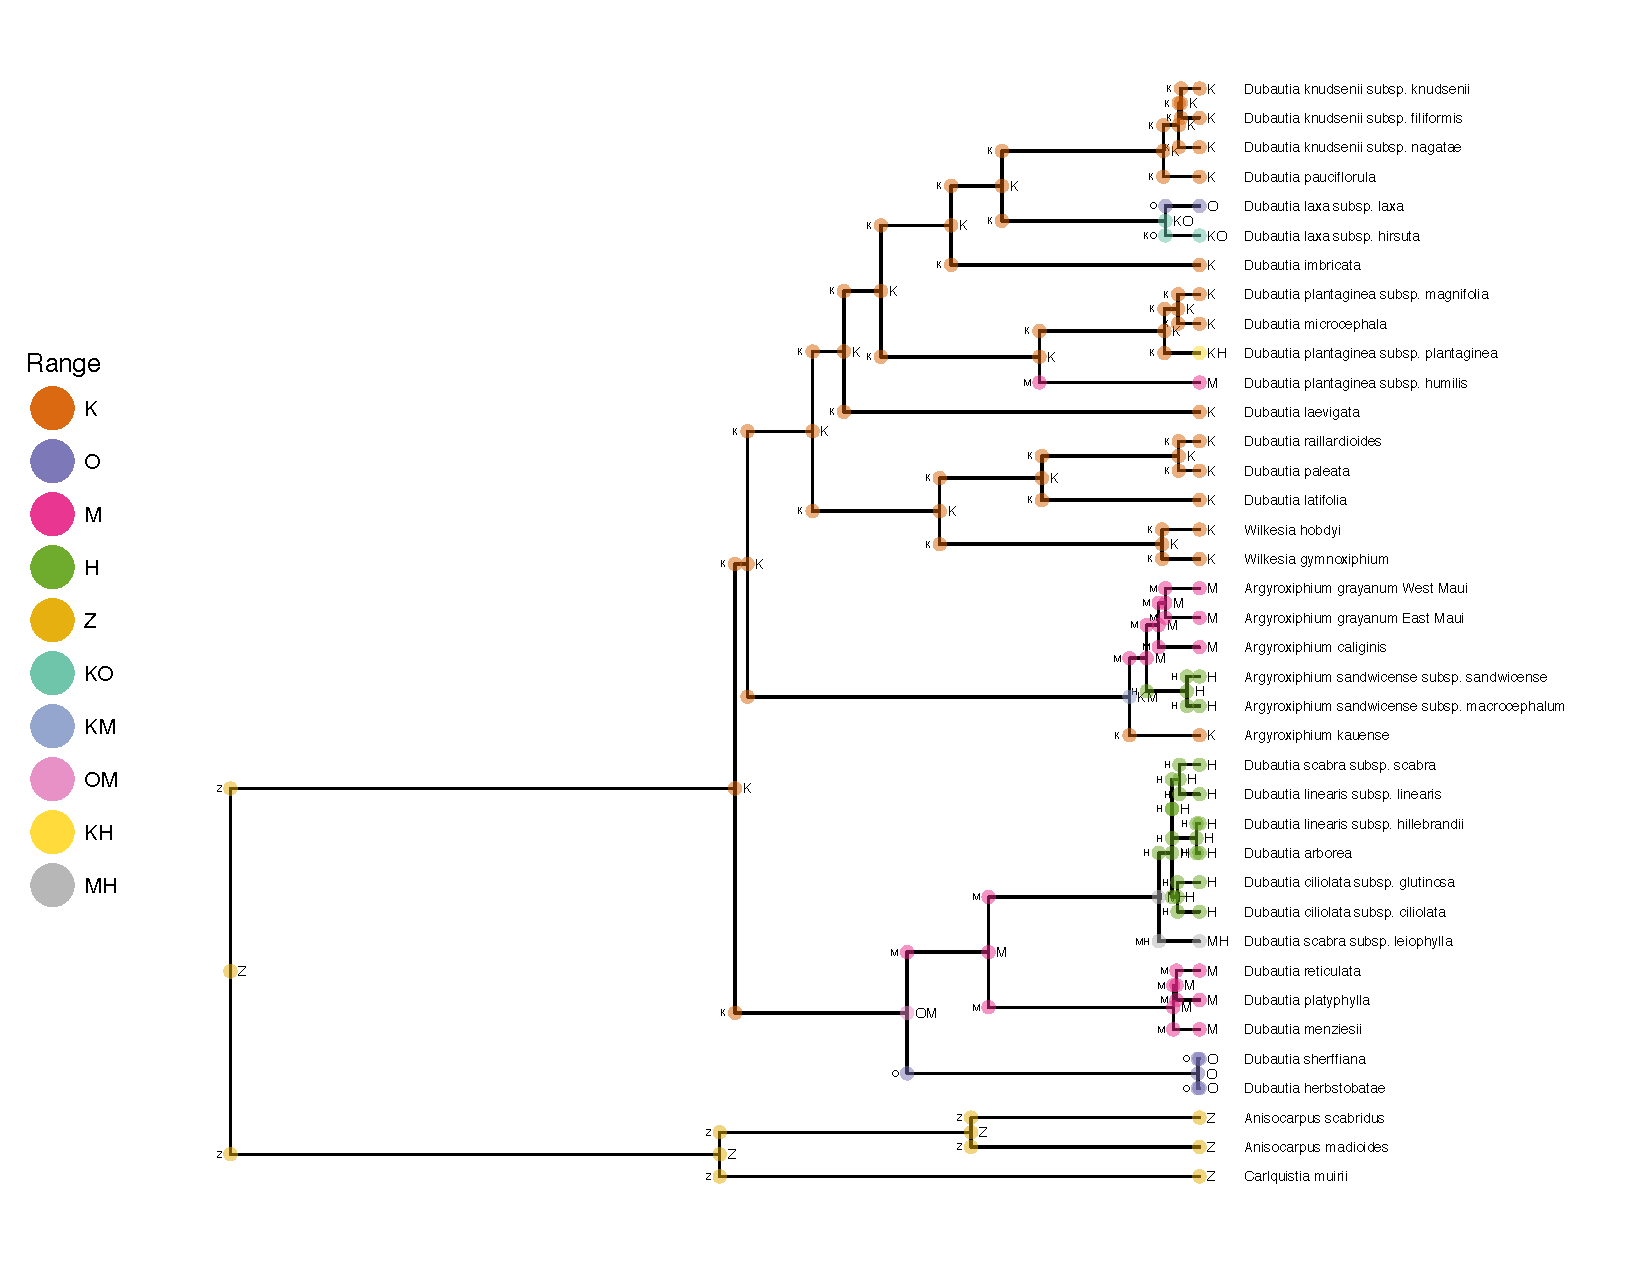
\includegraphics[width=0.8\textwidth]{figures/fig_epoch_phy_RevGadgets_ase.pdf} 
\caption{Joint estimate of phylogeny and biogeography, conditioning on paleogeography through the epoch model.}
\label{fig:epoch_phy}
\end{figure}

We see that simple analysis (Figure \ref{fig:simple_phy}) estimates the ancestral range at the root of the clade as Maui+Mainland (MZ).
This is unrealistic, both because of the extreme distance between those areas, but also the simple analysis estimates the root age to be 10.3 (HPD95\% 4.6, 15.0) Ma, well before Maui originated.
(Date estimates are reported in the {\tt simple\_phy.mcc.tre} and {\tt simple\_phy.model.log} files.)
The simple model also infers Kauai+Maui (KM) as the ancestral range of living silverswords and a crown age of 7.2 (HPD95\% 2.5, 13.5) Ma, which is impossibly ancient given the islands' ages.

The epoch analysis (Figure \ref{fig:epoch_phy}) produces more sensible ancestral range estimates, with Kauai being colonized first, and younger islands only being colonized as they become available.
The crown age of silverswords is estimated as 2.5 (HPD95\% 0.7, 4.3) Ma.
When comparing the results to the earlier fixed-phylogeny epoch results in Figure \ref{fig:epoch_RevGadgets_ase}, we recover a greater role for cladogenesis for the younger speciation events.
These two analyses only differ in terms of whether the phylogeny is fixed or estimated, so it is likely a result of phylogenetic error in the fixed tree.


\begin{figure}[!h]
\centering
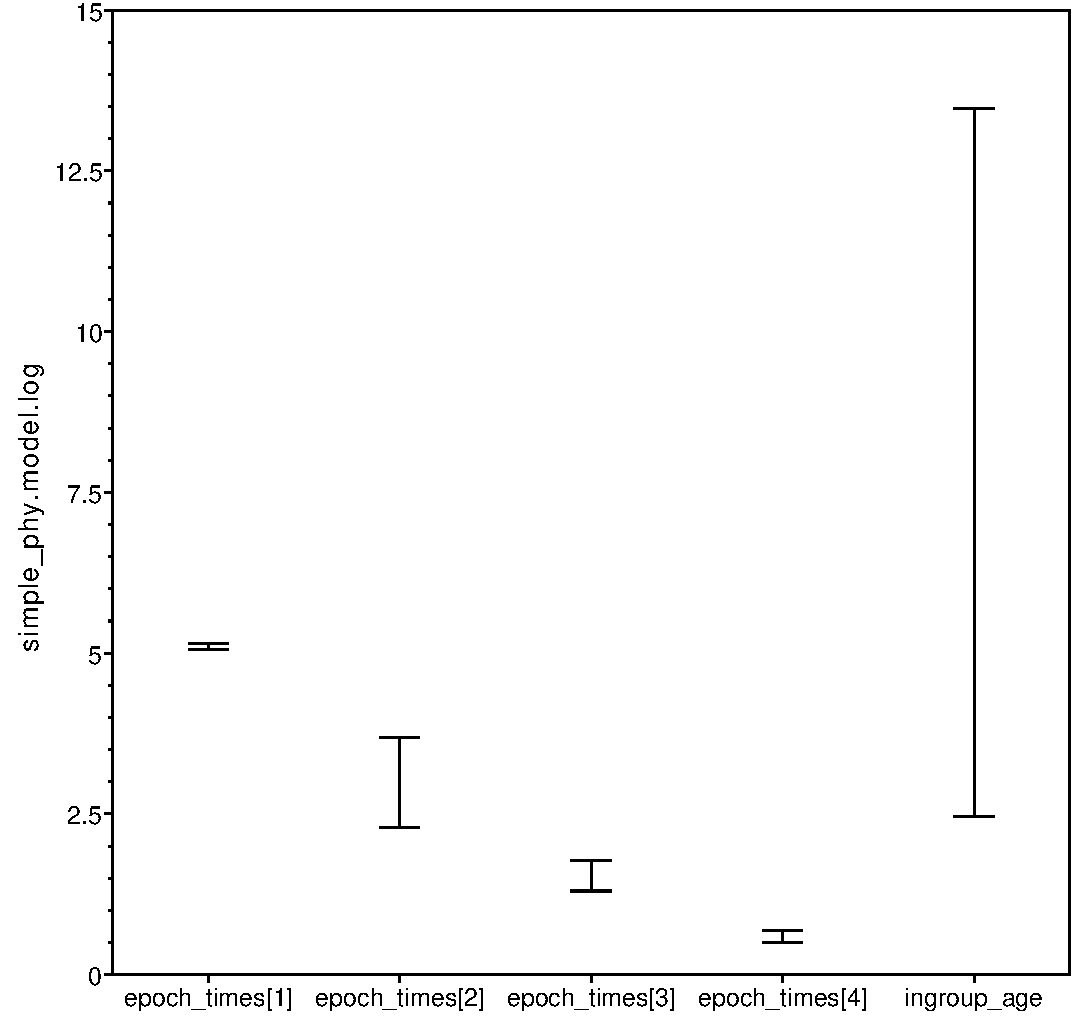
\includegraphics[width=0.4\textwidth]{figures/fig_simple_ages.pdf} 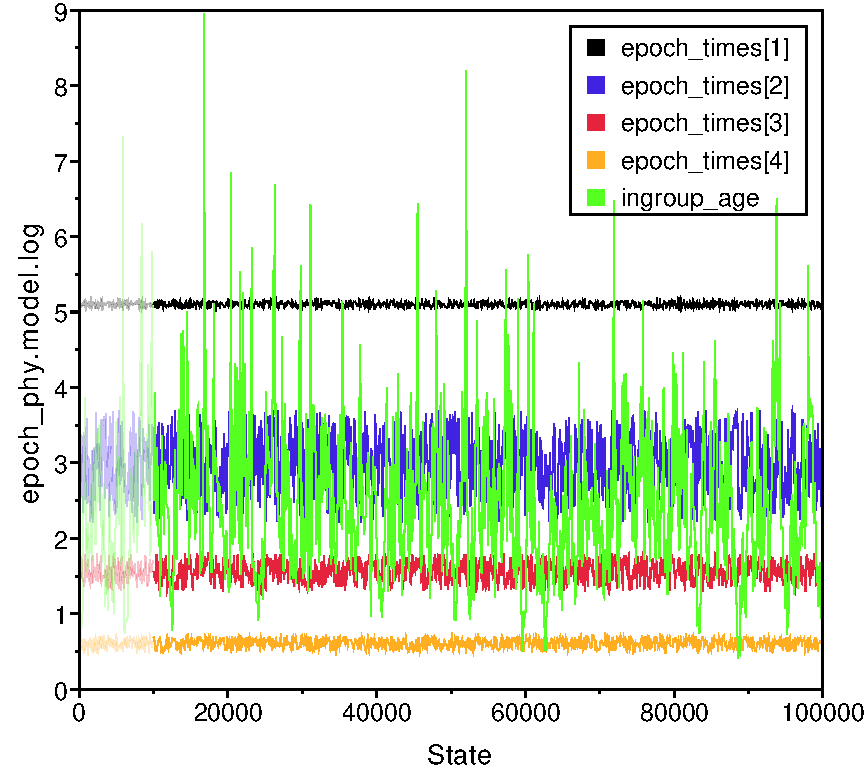
\includegraphics[width=0.4\textwidth]{figures/fig_epoch_ages.pdf} 

\caption{Plot of posterior samples for island ages and the origin time of living silverswords.
The colors black, blue, red, orange, and green correspond to the origination times of Kaui, Oahu, Maui, Hawaii, and the silversword clade, respectively.
The left panel ignores paleogeography, allowing silverswords to originate well before the formation of Kauai ({\tt epoch\_times[1]}).
The right panel conditions of paleogeography, which prefers a silversword crown age that follows the formation of Kauai.}
\label{fig:epoch_ages}
\end{figure}


In Tracer, one can look at the sampled posterior of island ages in comparison the origination time of crown silverswords (Figure \ref{fig:epoch_ages}).
The left panel shows the simple analysis, where crown silverswords often originate before the formation of Kauai.
The right panel shows that crown silverswords probably originated before the formation of Maui, but after the formation of Kauai.

\begin{table}[!h]
\centering
\begin{tabular}{c|cccc}
Model       & $P(a_s>a_K)$ & $P(a_s>a_O)$ & $P(a_s>a_M)$ & $P(a_s>a_H)$ \\ \hline
simple & 0.72 & 0.94 & 0.99 & 1.00 \\
epoch & 0.02 & 0.26 & 0.84 & 0.99 \\
\end{tabular}
\caption{Posterior probability that the age of crown silverswords ($a_s$) is older than the origination times of K, O, M, and H ($a_K, a_O, a_M, a_H$, respectively). The ``simple'' model (Left) ignores paleogeography while the ``epoch'' model (Right) conditions on it.}
\label{tab:epoch_ages}
\end{table}

By tabulating the results of the deterministic variable {\tt ingroup\_older\_island}, we measure the posterior probability that crown silverswords originated before or after each particular epoch in the model (Table \ref{tab:epoch_ages}).
Treating $P=0.95$ as significant support for an evolutionary outcome, the epoch model produces strong support that crown silverswords originated after the formation of Kauai, $P(a_s > a_K) = 0.02 < 1-0.95$ and weak support that they originated after the formation of Oahu, $P(a_s > a_O) = 0.26 > 1-0.95$.


\newpage
